\documentclass[aspectratio=169, 12pt]{beamer}

% ── Theme & Colors ──────────────────────────────────────────────────
\usetheme{default}
\usecolortheme{default}
\setbeamercolor{background canvas}{bg=black}
\setbeamercolor{normal text}{fg=white}
\setbeamercolor{frametitle}{fg=white}
\setbeamercolor{title}{fg=white}
\setbeamercolor{subtitle}{fg=gray!70}
\setbeamercolor{item}{fg=cyan!70}
\setbeamercolor{subitem}{fg=cyan!50}
\setbeamertemplate{navigation symbols}{}
\setbeamertemplate{footline}{}
\setbeamerfont{frametitle}{size=\Large, series=\bfseries}
\setbeamerfont{title}{size=\huge, series=\bfseries}

% ── Packages ────────────────────────────────────────────────────────
\usepackage{tikz}
\usetikzlibrary{arrows.meta, positioning, calc, decorations.pathmorphing, fit, shapes.geometric}
\usepackage{fontspec}
\usepackage{amsmath, amssymb}
\usepackage{graphicx}
\usepackage{xcolor}

% ── Custom colors ───────────────────────────────────────────────────
\definecolor{r3blue}{HTML}{4FC3F7}
\definecolor{h3green}{HTML}{81C784}
\definecolor{c3orange}{HTML}{FFB74D}
\definecolor{c3red}{HTML}{EF5350}
\definecolor{dimgray}{HTML}{666666}
\definecolor{accentpink}{HTML}{F48FB1}
\definecolor{accentpurple}{HTML}{CE93D8}
\definecolor{dopamine}{HTML}{FF7043}
\definecolor{serotonin}{HTML}{7E57C2}
\definecolor{opioid}{HTML}{26A69A}
\definecolor{norepinephrine}{HTML}{FFA726}

\begin{document}

% ════════════════════════════════════════════════════════════════════
% PAGE 1: Architecture Overview
% ════════════════════════════════════════════════════════════════════
\begin{frame}
\frametitle{Musical Intelligence \textemdash\ A Computational Brain for Music}

\begin{columns}[T]

% ── LEFT: Diagram ──────────────────────────────────────────────────
\begin{column}{0.52\textwidth}
\vspace{-0.3cm}
\centering
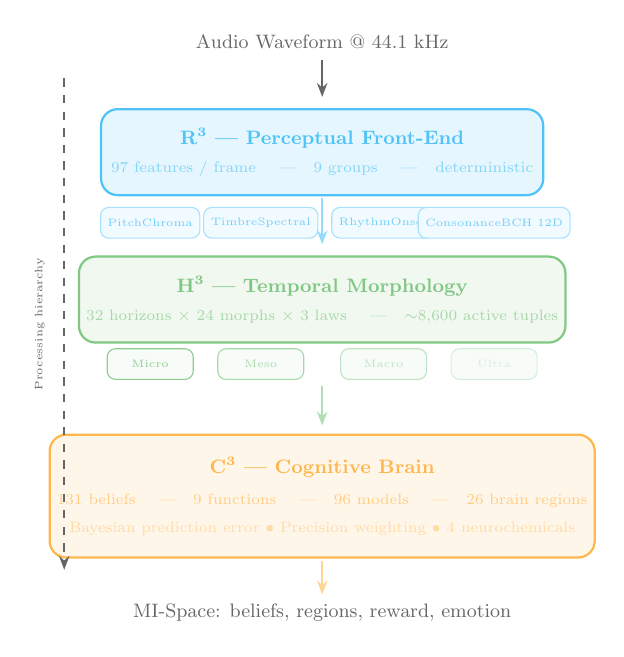
\begin{tikzpicture}[
    scale=0.78, transform shape,
    layer/.style={rounded corners=6pt, draw=white, thick, minimum width=7.2cm, minimum height=1.4cm, align=center, font=\small\bfseries},
    arrow/.style={-{Stealth[length=5pt]}, thick, white},
    label/.style={font=\tiny, text=dimgray, align=left}
]

% Audio input
\node[font=\small, text=dimgray] (audio) at (0, 7.6) {Audio Waveform @ 44.1 kHz};
\draw[arrow, dimgray] (0, 7.3) -- (0, 6.7);

% R³ Layer
\node[layer, fill=r3blue!15, draw=r3blue] (r3) at (0, 5.8)
    {\textcolor{r3blue}{R\textsuperscript{3} \textemdash\ Perceptual Front-End}\\[2pt]
     \textcolor{r3blue!70}{\normalfont\scriptsize 97 features / frame \quad|\quad 9 groups \quad|\quad deterministic}};

% R³ detail boxes
\node[rounded corners=3pt, draw=r3blue!50, fill=r3blue!8, minimum width=1.4cm, minimum height=0.5cm, font=\tiny, text=r3blue!80] at (-2.8, 4.65) {Pitch\\Chroma};
\node[rounded corners=3pt, draw=r3blue!50, fill=r3blue!8, minimum width=1.4cm, minimum height=0.5cm, font=\tiny, text=r3blue!80] at (-1.0, 4.65) {Timbre\\Spectral};
\node[rounded corners=3pt, draw=r3blue!50, fill=r3blue!8, minimum width=1.4cm, minimum height=0.5cm, font=\tiny, text=r3blue!80] at (1.0, 4.65) {Rhythm\\Onset};
\node[rounded corners=3pt, draw=r3blue!50, fill=r3blue!8, minimum width=1.4cm, minimum height=0.5cm, font=\tiny, text=r3blue!80] at (2.8, 4.65) {Consonance\\BCH 12D};

\draw[arrow, r3blue!60] (0, 5.05) -- (0, 4.3);

% H³ Layer
\node[layer, fill=h3green!12, draw=h3green] (h3) at (0, 3.4)
    {\textcolor{h3green}{H\textsuperscript{3} \textemdash\ Temporal Morphology}\\[2pt]
     \textcolor{h3green!70}{\normalfont\scriptsize 32 horizons \(\times\) 24 morphs \(\times\) 3 laws \quad|\quad \(\sim\)8{,}600 active tuples}};

% H³ horizon bar
\foreach \x/\lbl/\col in {-2.8/Micro/h3green!90, -1.0/Meso/h3green!70, 1.0/Macro/h3green!50, 2.8/Ultra/h3green!30} {
    \node[rounded corners=3pt, draw=\col, fill=h3green!6, minimum width=1.4cm, minimum height=0.5cm, font=\tiny, text=\col] at (\x, 2.35) {\lbl};
}

\draw[arrow, h3green!60] (0, 2.0) -- (0, 1.35);

% C³ Layer (larger)
\node[layer, fill=c3orange!12, draw=c3orange, minimum height=2.0cm] (c3) at (0, 0.2)
    {\textcolor{c3orange}{C\textsuperscript{3} \textemdash\ Cognitive Brain}\\[3pt]
     \textcolor{c3orange!70}{\normalfont\scriptsize 131 beliefs \quad|\quad 9 functions \quad|\quad 96 models \quad|\quad 26 brain regions}\\[2pt]
     \textcolor{c3orange!50}{\normalfont\scriptsize Bayesian prediction error \(\bullet\) Precision weighting \(\bullet\) 4 neurochemicals}};

% Output arrow
\draw[arrow, c3orange!60] (0, -0.85) -- (0, -1.4);
\node[font=\small, text=dimgray] at (0, -1.7) {MI-Space: beliefs, regions, reward, emotion};

% Side annotation: time arrow
\draw[arrow, dimgray, dashed] (-4.2, 7.0) -- (-4.2, -1.0);
\node[font=\tiny, text=dimgray, rotate=90] at (-4.6, 3.0) {Processing hierarchy};

\end{tikzpicture}
\end{column}

% ── RIGHT: Text ────────────────────────────────────────────────────
\begin{column}{0.45\textwidth}
\vspace{0.2cm}
\small

\textbf{\textcolor{white}{Three-layer neural architecture}} that transforms raw audio into a continuous stream of cognitive states\textemdash modeled after how the brain processes music.

\vspace{0.4cm}

\textcolor{r3blue}{\textbf{R\textsuperscript{3}}} \textcolor{white}{\textemdash\ Early Perception}\\[3pt]
{\footnotesize Frame-level feature extraction. Analogous to \textbf{cochlear nucleus} $\to$ \textbf{auditory cortex} (A1/A2). Deterministic, stateless, frozen.}

\vspace{0.35cm}

\textcolor{h3green}{\textbf{H\textsuperscript{3}}} \textcolor{white}{\textemdash\ Temporal Integration}\\[3pt]
{\footnotesize Multi-scale statistics over 32 time windows (23\,ms to 5\,min). Models how cortex builds \textbf{temporal expectations} via memory, forward prediction, and bidirectional integration.}

\vspace{0.35cm}

\textcolor{c3orange}{\textbf{C\textsuperscript{3}}} \textcolor{white}{\textemdash\ Cognitive Processing}\\[3pt]
{\footnotesize 131 belief variables updated via \textbf{predictive coding} (Friston, 2005). Maps to 26 anatomical regions (MNI152). Modulated by DA, 5-HT, NE, endogenous opioids.}

\vspace{0.35cm}

{\footnotesize\textcolor{dimgray}{756 Python files \(\bullet\) 448 supporting studies \(\bullet\) 634 effect sizes}}

\end{column}
\end{columns}
\end{frame}

% ════════════════════════════════════════════════════════════════════
% PAGE 2: C³ Belief Cycle & Brain Regions
% ════════════════════════════════════════════════════════════════════
\begin{frame}
\frametitle{C\textsuperscript{3} Belief Update Cycle \& Region Activation Map}

\begin{columns}[T]

% ── LEFT: Bayesian Cycle Diagram ───────────────────────────────────
\begin{column}{0.50\textwidth}
\vspace{-0.1cm}
\centering
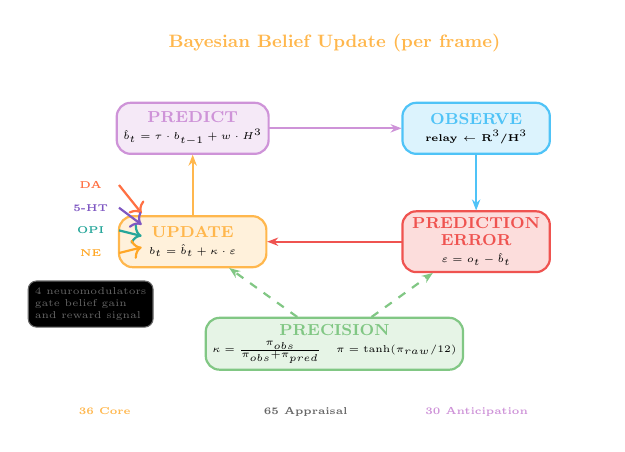
\begin{tikzpicture}[
    scale=0.72, transform shape,
    box/.style={rounded corners=5pt, draw=white, thick, minimum width=2.6cm, minimum height=0.9cm, align=center, font=\footnotesize\bfseries},
    arrow/.style={-{Stealth[length=4pt]}, thick},
]

% Title
\node[font=\small\bfseries, text=c3orange] at (0, 6.8) {Bayesian Belief Update (per frame)};

% Cycle nodes
\node[box, fill=accentpurple!20, draw=accentpurple] (predict) at (-2.5, 5.3) {\textcolor{accentpurple}{PREDICT}\\[-1pt]\tiny $\hat{b}_t = \tau \cdot b_{t-1} + w \cdot H^3$};

\node[box, fill=r3blue!20, draw=r3blue] (observe) at (2.5, 5.3) {\textcolor{r3blue}{OBSERVE}\\[-1pt]\tiny relay $\leftarrow$ R$^3$/H$^3$};

\node[box, fill=c3red!20, draw=c3red] (pe) at (2.5, 3.3) {\textcolor{c3red}{PREDICTION}\\[-1pt]\textcolor{c3red}{ERROR}\\[-1pt]\tiny $\varepsilon = o_t - \hat{b}_t$};

\node[box, fill=c3orange!20, draw=c3orange] (update) at (-2.5, 3.3) {\textcolor{c3orange}{UPDATE}\\[-1pt]\tiny $b_t = \hat{b}_t + \kappa \cdot \varepsilon$};

\node[box, fill=h3green!20, draw=h3green] (precision) at (0, 1.5) {\textcolor{h3green}{PRECISION}\\[-1pt]\tiny $\kappa = \frac{\pi_{obs}}{\pi_{obs} + \pi_{pred}}$\quad $\pi = \tanh(\pi_{raw}/12)$};

% Arrows
\draw[arrow, accentpurple] (predict) -- (observe);
\draw[arrow, r3blue] (observe) -- (pe);
\draw[arrow, c3red] (pe) -- (update);
\draw[arrow, c3orange] (update) -- (predict);
\draw[arrow, h3green, dashed] (precision) -- (update);
\draw[arrow, h3green, dashed] (precision) -- (pe);

% Neurochemical modulation
\node[font=\tiny\bfseries, text=dopamine] at (-4.3, 4.3) {DA};
\node[font=\tiny\bfseries, text=serotonin] at (-4.3, 3.9) {5-HT};
\node[font=\tiny\bfseries, text=opioid] at (-4.3, 3.5) {OPI};
\node[font=\tiny\bfseries, text=norepinephrine] at (-4.3, 3.1) {NE};
\draw[thick, dopamine, ->] (-3.8, 4.3) -- (-3.4, 3.8);
\draw[thick, serotonin, ->] (-3.8, 3.9) -- (-3.4, 3.6);
\draw[thick, opioid, ->] (-3.8, 3.5) -- (-3.4, 3.4);
\draw[thick, norepinephrine, ->] (-3.8, 3.1) -- (-3.4, 3.2);
\node[rounded corners=3pt, draw=dimgray, fill=black, font=\tiny, text=dimgray, align=left] at (-4.3, 2.2) {4 neuromodulators\\gate belief gain\\and reward signal};

% Belief types annotation
\node[font=\tiny, text=white, align=center] at (0, 0.3) {
\textcolor{c3orange}{\textbf{36 Core}} (full Bayesian PE) \quad
\textcolor{dimgray}{\textbf{65 Appraisal}} (observe) \quad
\textcolor{accentpurple}{\textbf{30 Anticipation}} (predict)
};

\end{tikzpicture}
\end{column}

% ── RIGHT: Brain Region Map ────────────────────────────────────────
\begin{column}{0.48\textwidth}
\vspace{-0.1cm}
\centering
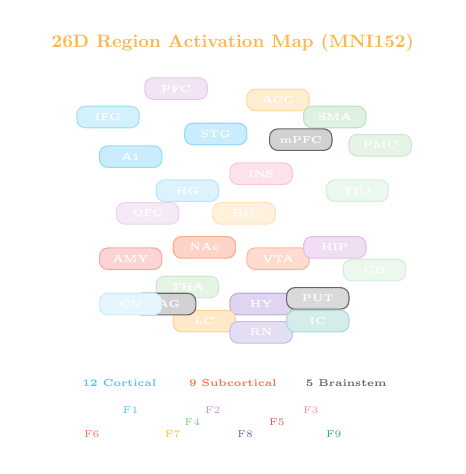
\begin{tikzpicture}[
    scale=0.72, transform shape,
    region/.style={rounded corners=3pt, minimum width=1.1cm, minimum height=0.38cm, font=\tiny\bfseries, align=center, inner sep=2pt},
]

% Title
\node[font=\small\bfseries, text=c3orange] at (0, 6.8) {26D Region Activation Map (MNI152)};

% Simplified brain outline (sagittal view)
\draw[white!30, thick, rounded corners=15pt] (-3.2, 2.5) -- (-2.8, 5.5) -- (-0.5, 6.2) -- (2.0, 5.8) -- (3.2, 4.5) -- (3.0, 2.8) -- (1.5, 1.8) -- (-0.5, 1.5) -- (-2.5, 1.8) -- cycle;

% Cortical (12) - upper brain
\node[region, fill=r3blue!30, draw=r3blue!60, text=white] (a1) at (-1.8, 4.8) {A1};
\node[region, fill=r3blue!30, draw=r3blue!60, text=white] (stg) at (-0.3, 5.2) {STG};
\node[region, fill=r3blue!25, draw=r3blue!50, text=white] (ifg) at (-2.2, 5.5) {IFG};
\node[region, fill=accentpurple!25, draw=accentpurple!50, text=white] (pfc) at (-1.0, 6.0) {PFC};
\node[region, fill=c3orange!25, draw=c3orange!50, text=white] (acc) at (0.8, 5.8) {ACC};
\node[region, fill=h3green!25, draw=h3green!50, text=white] (sma) at (1.8, 5.5) {SMA};
\node[region, fill=h3green!20, draw=h3green!40, text=white] (pmc) at (2.6, 5.0) {PMC};
\node[region, fill=accentpink!25, draw=accentpink!50, text=white] (ins) at (0.5, 4.5) {INS};
\node[region, fill=accentpurple!20, draw=accentpurple!40, text=white] (ofc) at (-1.5, 3.8) {OFC};
\node[region, fill=r3blue!20, draw=r3blue!40, text=white] (hg) at (-0.8, 4.2) {HG};
\node[region, fill=h3green!15, draw=h3green!30, text=white] (tpj) at (2.2, 4.2) {TPJ};
\node[region, fill=dimgray!30, draw=dimgray, text=white] (mpc) at (1.2, 5.1) {mPFC};

% Subcortical (9) - middle
\node[region, fill=dopamine!30, draw=dopamine!60, text=white] (nac) at (-0.5, 3.2) {NAc};
\node[region, fill=dopamine!25, draw=dopamine!50, text=white] (vta) at (0.8, 3.0) {VTA};
\node[region, fill=c3red!25, draw=c3red!50, text=white] (amy) at (-1.8, 3.0) {AMY};
\node[region, fill=accentpurple!30, draw=accentpurple!60, text=white] (hip) at (1.8, 3.2) {HIP};
\node[region, fill=c3orange!20, draw=c3orange!40, text=white] (bg) at (0.2, 3.8) {BG};
\node[region, fill=h3green!20, draw=h3green!40, text=white] (tha) at (-0.8, 2.5) {THA};
\node[region, fill=h3green!15, draw=h3green!30, text=white] (cb) at (2.5, 2.8) {CB};
\node[region, fill=serotonin!25, draw=serotonin!50, text=white] (hy) at (0.5, 2.2) {HY};
\node[region, fill=dimgray!25, draw=dimgray, text=white] (put) at (1.5, 2.3) {PUT};

% Brainstem (5) - lower
\node[region, fill=norepinephrine!25, draw=norepinephrine!50, text=white] (lc) at (-0.5, 1.9) {LC};
\node[region, fill=serotonin!20, draw=serotonin!40, text=white] (rn) at (0.5, 1.7) {RN};
\node[region, fill=dimgray!30, draw=dimgray, text=white] (pag) at (-1.2, 2.2) {PAG};
\node[region, fill=opioid!20, draw=opioid!40, text=white] (ic) at (1.5, 1.9) {IC};
\node[region, fill=r3blue!15, draw=r3blue!30, text=white] (cn) at (-1.8, 2.2) {CN};

% Legend
\node[font=\tiny, text=r3blue, align=left] at (-2.0, 0.8) {\textbf{12 Cortical}};
\node[font=\tiny, text=dopamine, align=left] at (0.0, 0.8) {\textbf{9 Subcortical}};
\node[font=\tiny, text=dimgray, align=left] at (2.0, 0.8) {\textbf{5 Brainstem}};

% 9 Functions annotation
\node[font=\tiny, text=white, align=center, text width=7cm] at (0, 0.1) {
\textcolor{r3blue}{F1} Sensory \(\bullet\)
\textcolor{accentpurple}{F2} Prediction \(\bullet\)
\textcolor{accentpink}{F3} Attention \(\bullet\)
\textcolor{h3green}{F4} Memory \(\bullet\)
\textcolor{c3red}{F5} Emotion\\
\textcolor{dopamine}{F6} Reward \(\bullet\)
\textcolor{c3orange}{F7} Motor \(\bullet\)
\textcolor{serotonin}{F8} Learning \(\bullet\)
\textcolor{opioid}{F9} Social
};

\end{tikzpicture}
\end{column}

\end{columns}
\end{frame}

% ════════════════════════════════════════════════════════════════════
% PAGE 3: Validation & Empirical Grounding
% ════════════════════════════════════════════════════════════════════
\begin{frame}
\frametitle{Empirical Validation \& Evidence Base}

\begin{columns}[T]

% ── LEFT: Validation Pipeline Diagram ──────────────────────────────
\begin{column}{0.50\textwidth}
\vspace{-0.1cm}
\centering
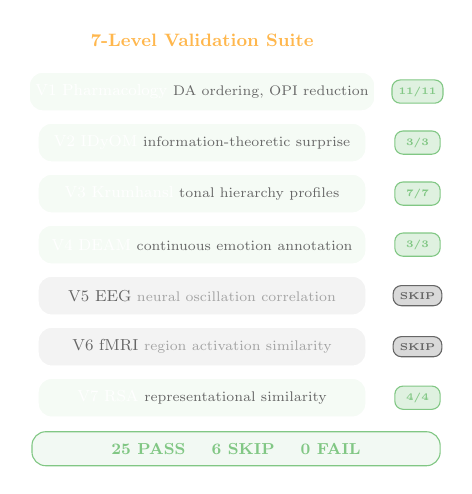
\begin{tikzpicture}[
    scale=0.72, transform shape,
    vbox/.style={rounded corners=5pt, draw=white, thick, minimum width=5.8cm, minimum height=0.7cm, align=center, font=\footnotesize},
    pass/.style={rounded corners=3pt, fill=h3green!25, draw=h3green, text=h3green, font=\tiny\bfseries, minimum width=0.8cm},
    skip/.style={rounded corners=3pt, fill=dimgray!25, draw=dimgray, text=dimgray, font=\tiny\bfseries, minimum width=0.8cm},
    arrow/.style={-{Stealth[length=4pt]}, thick, white!50},
]

% Title
\node[font=\small\bfseries, text=c3orange] at (0, 7.2) {7-Level Validation Suite};

% V1
\node[vbox, fill=h3green!8] (v1) at (0, 6.3) {\textcolor{white}{V1 Pharmacology} \textcolor{dimgray}{\scriptsize DA ordering, OPI reduction}};
\node[pass] at (3.8, 6.3) {11/11};

% V2
\node[vbox, fill=h3green!8] (v2) at (0, 5.4) {\textcolor{white}{V2 IDyOM} \textcolor{dimgray}{\scriptsize information-theoretic surprise}};
\node[pass] at (3.8, 5.4) {3/3};

% V3
\node[vbox, fill=h3green!8] (v3) at (0, 4.5) {\textcolor{white}{V3 Krumhansl} \textcolor{dimgray}{\scriptsize tonal hierarchy profiles}};
\node[pass] at (3.8, 4.5) {7/7};

% V4
\node[vbox, fill=h3green!8] (v4) at (0, 3.6) {\textcolor{white}{V4 DEAM} \textcolor{dimgray}{\scriptsize continuous emotion annotation}};
\node[pass] at (3.8, 3.6) {3/3};

% V5
\node[vbox, fill=dimgray!8] (v5) at (0, 2.7) {\textcolor{dimgray}{V5 EEG} \textcolor{dimgray!60}{\scriptsize neural oscillation correlation}};
\node[skip] at (3.8, 2.7) {SKIP};

% V6
\node[vbox, fill=dimgray!8] (v6) at (0, 1.8) {\textcolor{dimgray}{V6 fMRI} \textcolor{dimgray!60}{\scriptsize region activation similarity}};
\node[skip] at (3.8, 1.8) {SKIP};

% V7
\node[vbox, fill=h3green!8] (v7) at (0, 0.9) {\textcolor{white}{V7 RSA} \textcolor{dimgray}{\scriptsize representational similarity}};
\node[pass] at (3.8, 0.9) {4/4};

% Arrows between
\foreach \i/\j in {v1/v2, v2/v3, v3/v4, v4/v5, v5/v6, v6/v7} {
    \draw[arrow] (\i) -- (\j);
}

% Summary bar
\node[rounded corners=5pt, draw=h3green, fill=h3green!10, minimum width=7.2cm, minimum height=0.6cm, font=\footnotesize\bfseries, text=h3green] at (0.6, 0.0) {25 PASS \quad 6 SKIP \quad 0 FAIL};

\end{tikzpicture}
\end{column}

% ── RIGHT: Evidence Numbers & Meta-analysis ────────────────────────
\begin{column}{0.47\textwidth}
\vspace{0.1cm}

\textbf{\textcolor{c3orange}{Literature Base}}\\[6pt]
{\footnotesize
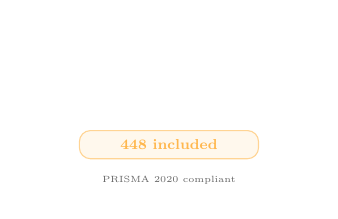
\begin{tikzpicture}[scale=0.65, transform shape]
    % PRISMA funnel
    \node[rounded corners=4pt, draw=white!50, fill=white!5, minimum width=5.5cm, minimum height=0.55cm, font=\footnotesize, text=white] (s1) at (0, 4.5) {2,847 studies screened};
    \node[rounded corners=4pt, draw=white!40, fill=white!5, minimum width=4.5cm, minimum height=0.55cm, font=\footnotesize, text=white] (s2) at (0, 3.5) {612 assessed};
    \node[rounded corners=4pt, draw=c3orange!60, fill=c3orange!10, minimum width=3.5cm, minimum height=0.55cm, font=\footnotesize\bfseries, text=c3orange] (s3) at (0, 2.5) {448 included};
    \draw[white!30, thick] (-2.3, 4.15) -- (-1.8, 3.85);
    \draw[white!30, thick] (2.3, 4.15) -- (1.8, 3.85);
    \draw[white!30, thick] (-1.8, 3.15) -- (-1.4, 2.85);
    \draw[white!30, thick] (1.8, 3.15) -- (1.4, 2.85);
    % Numbers
    \node[font=\tiny, text=dimgray] at (0, 1.8) {PRISMA 2020 compliant};
\end{tikzpicture}
}

\vspace{0.1cm}

{\footnotesize
\textcolor{white}{\textbf{1,116}} empirical claims extracted\\[3pt]
\textcolor{white}{\textbf{634}} effect sizes (random-effects meta-analysis)\\[3pt]
\textcolor{white}{\textbf{96}} computational models implemented\\[3pt]
\textcolor{white}{\textbf{416}} bibliography entries
}

\vspace{0.4cm}

\textbf{\textcolor{c3orange}{Core-4 Meta-Analysis}} {\scriptsize\textcolor{dimgray}{(Cohen's \textit{d})}}\\[6pt]
{\footnotesize
\begin{tikzpicture}[scale=0.65, transform shape]
    % Bar chart
    \foreach \y/\lbl/\val/\w/\col in {
        3/SPU (Sensory)/0.84/3.36/r3blue,
        2/STU (Temporal)/0.67/2.68/h3green,
        1/IMU (Integration)/0.53/2.12/accentpurple,
        0/ARU (Reward)/0.83/3.32/dopamine
    } {
        \fill[\col!40] (0, \y*0.8) rectangle (\w, \y*0.8+0.5);
        \draw[\col, thick] (0, \y*0.8) rectangle (\w, \y*0.8+0.5);
        \node[font=\tiny, text=white, anchor=west] at (0.1, \y*0.8+0.25) {\lbl};
        \node[font=\tiny\bfseries, text=\col, anchor=west] at (\w+0.15, \y*0.8+0.25) {\textit{d}=\val};
    }
    % Axis
    \draw[white!30, thin] (0, -0.15) -- (0, 3.0);
    \node[font=\tiny, text=dimgray] at (2, -0.4) {Effect size (Cohen's \textit{d})};
\end{tikzpicture}
}

\vspace{0.2cm}

{\scriptsize\textcolor{dimgray}{Evidence tiers: \textcolor{c3orange}{$\alpha$} mechanistic \(\bullet\) \textcolor{h3green}{$\beta$} integrative \(\bullet\) \textcolor{dimgray}{$\gamma$} speculative}}

\end{column}

\end{columns}
\end{frame}

\end{document}
